\documentclass[a4paper,oneside]{Tptesi2}

\usepackage[italian]{babel}
\usepackage{listings}
\usepackage{amsmath,amssymb}
\usepackage{verbatim}
\usepackage{indentfirst}
\usepackage[utf8]{inputenc}
\usepackage{subfigure}
\usepackage{algorithmic}
\usepackage{framed}
\usepackage{rotating}
\usepackage{cite}

\usepackage{multirow}

% Packages -----------------------------------------------------------------------
%\usepackage{amsthm}
%\usepackage{amsmath}          % Non necessario se usi TPTESI2 perche' gia` incluso
%\usepackage[dvips]{graphicx}  % Non necessario se usi TPTESI2 perche' gia` incluso
%\usepackage{url} %non usare se si usa hyperref


\newcommand{\mr}{\emph{motore di ricerca}}
\newcommand{\Mr}{\emph{Motore di ricerca}}
\newcommand{\ws}{Web~service }


% Use a small font for the verbatim environment
\makeatletter  % makes '@' an ordinary character
\renewcommand{\verbatim@font}{%
  \ttfamily\footnotesize\catcode`\<=\active\catcode`\>=\active%
}
\makeatother   % makes '@' a special symbol again
%
% Simboli Matematici -------------------------------------------------------------
%\newcommand{\h}{\mathcal{H}_\infty} % scorciatoia per sequenza usata spesso
% Definizioni & Teoremi ----------------------------------------------------------
\newtheorem{teorema}{Teorema}[chapter]
\newtheorem{corollario}[teorema]{Corollario}
\newtheorem{lemma}[teorema]{Lemma}
%\theoremstyle{definition}
\newtheorem{definizione}{Definizione}[chapter]
\newtheorem{proposizione}[definizione]{Proposizione}
% Formattazione Figure -----------------------------------------------------------
\setcounter{topnumber}{3}
\setcounter{totalnumber}{3}
\def\topfraction{1}
\def\textfraction{0}
% Fuzz ---------------------------------------------------------------------------
%\hfuzz10cm %Non scassare linee che escono dal bordo
% Frontespizio -------------------------------------------------------------------
       \title{Ricerca di grafemi in manoscritti}
       \author{Marco Benelli}
       \titolocorso{Ingegneria Informatica}
       \chair{Prof. Simone Marinai \\ }
       \numberofmembers{1} %numero dei relatori
       \degreeyear{2019/2020}
       %\numerocorrelatori{0} %numero dei correlatori
       %\correlatori{insert correlators\ldots} % i correlatori separati da \\

%
% ---- Inclusioni (vedi piu` sotto per il comando "include" --------------
%\includeonly {introduzione,chapter1, chapter2}
%\includeonly {chapter1, chapter2, chapter3, chapter4, chapter5, chapter6}
%\includeonly{chapter6}
%
\hypersetup{%
%  pdfpagemode=FullScreen,%
  plainpages=false,%
  breaklinks,%
  pdftitle={},%
  pdfauthor={},%
  pdfsubject={},%
  pdfkeywords={},%
  colorlinks=false}

\begin{document}

\frontmatter

%\hyphenation{}
%
\pagestyle{headings} % rende attive le impostazioni sulla testata!
%
\maketitle % crea il frontespizio (ricordati di copiare "stemma.eps" nella tua directory)
%
%
%\pagenumbering{roman}
\tableofcontents % inserisce indice generale
\cleardoublepage
%\addcontentsline{toc}{chapter}{Elenco delle figure}
%\listoffigures   % inserisce indice figure
%\addcontentsline{toc}{chapter}{Elenco delle tabelle}
%\listoftables    % inserisce indice tabelle
%\addcontentsline{toc}{chapter}{Elenco degli algoritmi}
%\listofalgorithms
%
%--------------- Inizio del testo vero e proprio
%

%\cleardoublepage
%\pagenumbering{arabic}
%\input{files/ringraziamenti}
\frontmatter
\chapter{Introduzione}\label{ch:introduzione}

Negli ultimi anni siamo andati verso l'automatizzazione di sempre pi\`u compiti, dai pi\`u semplici ai pi\`u complessi e con vari gradi di successo. Alcuni di questi compiti vengono lasciati ai computer perch\'e troppo complessi per gli umani; altri invece risultano elementari alle persone, ma si incontrano difficolt\`a nell'implementarli in maniera automatica. Si potrebbe quindi pensare che sia illogico cercare di automatizzare qualcosa che le persone trovano naturale, ma si sbaglierebbe. Infatti i computer hanno numerosi vantaggi rispetto alle persone: sono pi\`u veloci per le operazioni basilari e il loro tempo ha meno valore.

Una delle operazioni che alle persone riesce in maniera naturale \`e la lettura di documenti a partire da immagini degli stessi. Per un programma questo \`e un compito molto difficile, basti pensare ai CAPTCHA che si trovavano maggiormente fino a pochi anni fa.

Per questo progetto lo scopo non \`e la lettura, ma solamente il riconoscimento di alcuni grafemi in immagini di manoscritti medievali. Un grafema \`e un segno grafico a cui \`e associata una lettera; questa associazione non \`e biunivoca, infatti pi\`u grafemi possono corrispondere alla stessa lettera se quella lettera si pu\`o scrivere in pi\`u modi.

Questo pu\`o risultare utile perch\'e, conoscendo l'evoluzione della calligrafia nel corso dei secoli, il diverso stile di scrittura di una lettera ci pu\`o aiutare nella datazione dei manoscritti.

Il programma \`e scritto in \emph{Python} e le librerie che sono state usate sono:
\emph{OpenCV}\cite{opencv_library} per le operazioni sulle immagini;
\emph{numpy}\cite{oliphant2006guide, van2011numpy} per le operazioni sulle array;
\emph{matplotlib}\cite{Hunter:2007} per visualizzare alcuni grafici;
\emph{scipy}\cite{2020SciPy-NMeth} per alcune operazioni particolari.

Ci\`o che faremo per raggiungere il nostro obiettivo \`e, a partire da un grafema di riferimento, estrarre dal testo quelli simili. Per l'estrazione dei caratteri si useranno proiezioni ortogonali e componenti connesse, e per valutare la somiglianza, invece, sar\`a impiegato l'indice di Jaccard. Vedremo poi come poter introdurre dell'interattivit\`a nel programma facendo scegliere all'utente se una determinata immagine rappresenta il grafema desiderato. Per tutte queste modalit\`a saranno fatti degli esperimenti per valutarne l'efficienza.

\mainmatter
\chapter{Approccio proposto}%\label{ch:chapter1}

L'approccio che \`e stato utilizzato si articola in pi\`u fasi che andremo a vedere nel corso di questo capitolo.

\section{Preprocessing}

Le immagini di partenza sono lette e convertite in immagini in scala di grigi usando \emph{OpenCV} (gli scan di partenza sono a colori).

Successivamente vengono binarizzate, ovvero passano da essere in scala di grigi ad essere in bianco e nero. Per la binarizzazione viene usata la soglia di 128, quindi tutti i pixel che hanno un valore $<128$ diventano neri, mentre quelli con un valore $\ge128$ diventano bianchi.

Il valore di soglia (128), pu\`o chiaramente essere cambiato. \`E stato scelto il valore di 128 poich\'e a met\`a fra 0 e 255, che \`e il massimo valore che pu\`o avere un pixel in scala di grigi nella risoluzione a 8 bit per ogni pixel. Inoltre il valore di 128 sembra funzionare bene per le immagini di nostro interesse.

Se si dovessero analizzare altri scan, si pu\`o aggiustare il valore di soglia o addirittura cambiare il metodo di binarizzazione usandone uno pi\`u raffinato.

\section{Segmentazione}\label{sect:segmentation}

Per segmentazione si intende la separazione del documento nei vari caratteri che lo compongono. Questo processo non pu\`o essere perfetto se non si conosce la lingua che si vuole leggere, poich\'e in certi casi nella scrittura a mano possono esserci dei tratti ambigui che si riescono a capire solamente guardando il contesto della parola o addirittura della frase.

\subsection{Separazione delle righe}

Prima di separare i caratteri di una parola dobbiamo separare il documento nelle righe di testo che lo compongono. Per fare ci\`o, possiamo contare, in ciascuna riga di pixel, quanti sono neri e prendere i minimi relativi come punti di separazione. Nella figura \ref{fig:horiz_proj} \`e riportato il grafico del numero di pixel neri delle righe in una pagina.

\begin{figure}
%    \centering
    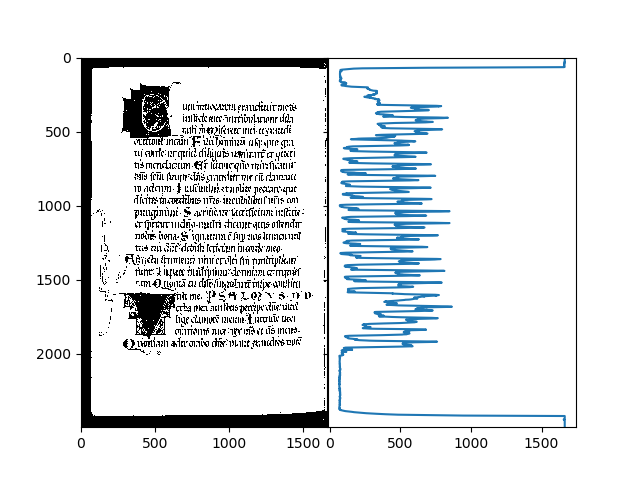
\includegraphics[width=\textwidth]{figures/horizontal-projection.png}
    \caption{A sinistra l'immagine binarizzata, a destra il conto dei pixel neri in ciascuna riga dell'immagine (sulle ordinate il numero della riga e sulle ascisse il numero di pixel).}
    \label{fig:horiz_proj}
\end{figure}

Guardando attentamente la figura \ref{fig:horiz_proj}, si nota che i minimi relativi del grafico sono molti di pi\`u delle righe di testo e, in particolare, molti minimi vanno a cascare nel mezzo di una riga. Questo \`e un problema che possiamo risolvere con delle finestre scorrevoli.

\subsubsection{Media mobile}

Per calcolare la media mobile possiamo utilizzare una finestra scorrevole. Applicare una finestra scorrevole di grandezza $n$ ad un array di numeri, significa sostituire ad ogni valore, la media degli $n$ valori pi\`u vicini. Questo processo tende a far diminuire la differenza fra un elemento e il successivo e porta ad eliminare molti massimi e minimi relativi.

Nella figura \ref{fig:all_smooth} possiamo vedere come la finestra scorrevole agisce sull'array di partenza. In particolare in figura \ref{fig:horiz_proj_smooth} possiamo vedere come i minimi relativi adesso si trovano sempre fra due righe di testo.

\begin{figure}
    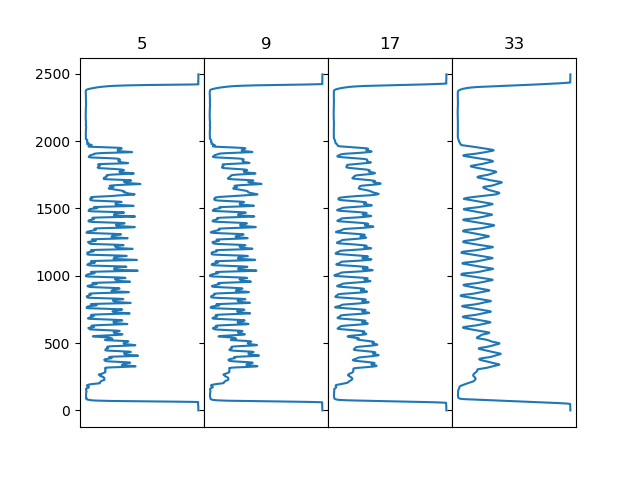
\includegraphics[width=\textwidth]{figures/all-smooth.png}
    \caption{I grafici relativi a finestre scorrevoli di varia grandezza (sopra ciascun grafico \`e segnata la dimensione della finestra).}
    \label{fig:all_smooth}
\end{figure}

\begin{figure}
    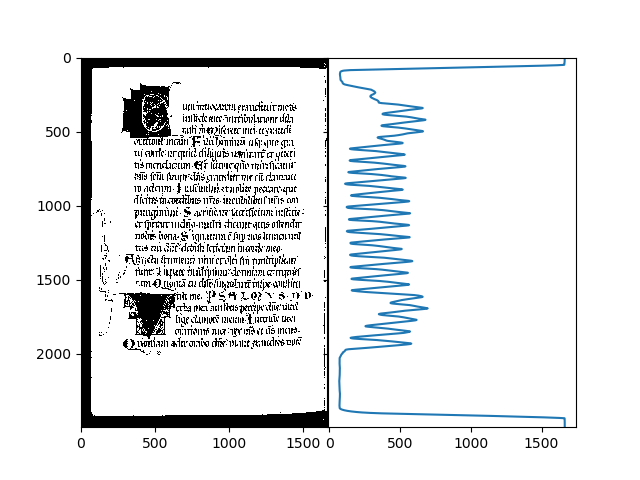
\includegraphics[width=\textwidth]{figures/horizontal-projection-smoothed.png}
    \caption{L'immagine di partenza affiancata alla proiezione a cui \`e stata applicata una finestra scorrevole di 33.}
    \label{fig:horiz_proj_smooth}
\end{figure}

\subsection{Separazione dei caratteri}

Nonostante non si possa sperare di separare i caratteri con esattezza, possiamo comunque separare le varie righe e fare delle ipotesi sui punti in cui finisce un carattere e inizia il successivo usando lo stesso metodo visto per separare le righe.

In figura \ref{fig:vert_proj_smooth} si vede una riga di testo e la proiezione verticale corrispondente ad una finestra scorrevole di dimensione 9; mentre nella figura \ref{fig:sectioned_row} \`e presente la stessa riga con delle barre verticali in corrispondenza dei minimi relativi.

\begin{figure}
    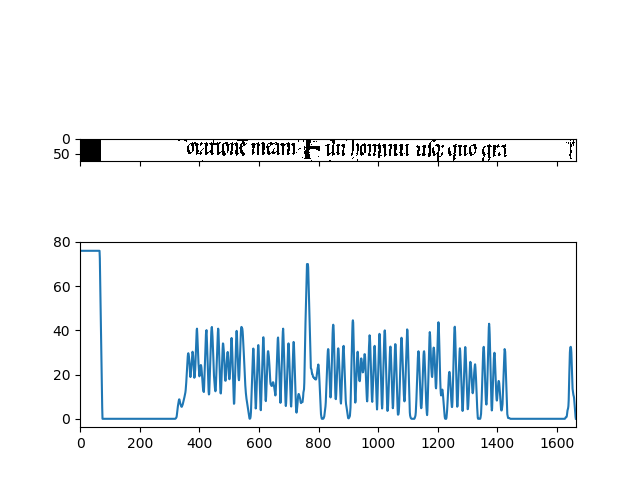
\includegraphics[width=\textwidth]{figures/vertical-projection-smooth.png}
    \caption{Sopra la riga di testo e sotto il grafico della proiezione verticale a cui \`e stata applicata una finestra scorrevole di dimensione 9.}
    \label{fig:vert_proj_smooth}
\end{figure}

\begin{figure}
    
\includegraphics[width=\textwidth]{figures/Bodmer 30_012v_large.jpg_sectioned_row_10.jpg}
    \caption{Una riga di testo sezionata verticalmente.}
    \label{fig:sectioned_row}
\end{figure}

Come si vede dalla figura \ref{fig:sectioned_row} e come avevamo predetto all'inizio del capitolo, la separazione dei caratteri non \`e stata perfetta. Nonostante ci\`o, i corretti punti di divisione sono tutti stati individuati, l'unico problema \`e che sono stati individuati anche punti di divisione incorretti. Questo non sar\`a comunque un problema come vedremo nel capitolo successivo.

\section{Estrazione delle lettere}

Per estrarre le lettere da una riga di testo come quella in figura \ref{fig:sectioned_row}, dobbiamo guardare non solo i rettangoli di pixel che sono delimitati da due minimi nella proiezione verticale, ma dobbiamo anche guardare gruppi di 2 o 3 rettangoli contigui. Molte lettere, infatti, sono separate da 1 linea verticale e alcune, come la \emph{m}, anche da 2.

Adesso che abbiamo una porzione di immagine rettangolare come quella in figura \ref{fig:unpolished_letter}, dobbiamo estrarre la lettera vera e propria. Infatti, si possono vedere dei pezzi delle lettere confinanti che sono entrati nel rettangolo corrispondente alla nostra lettera.

\begin{figure}
    \centering
    \frame{
\includegraphics{figures/Bodmer 30_012v_large.jpgstaticd1.png(7, 56, 2).png}}
    \caption{Un rettangolo dell'immagine contenente la lettera \emph{d}.}
    \label{fig:unpolished_letter}
\end{figure}

\subsection{Componenti connesse}

Per prima cosa dobbiamo individuare le componenti connesse dell'immagine. Consideriamo un grafo non orientato che ha come vertici i pixel neri e come archi quelli andiamo adesso a definire. Possiamo dire che esiste un arco fra due vertici, se i pixel (poligoni) corrispondenti condividono un lato (connessione a 4) oppure se condividono un lato o un vertice (connessione a 8). La figura \ref{fig:connectivity} mostra i due diversi tipi di connessione.

\begin{figure}
    \centering
    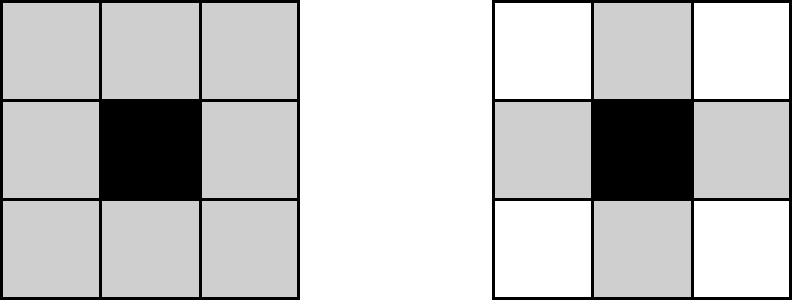
\includegraphics[width=0.5\textwidth]{figures/Sasiedztwa_4_8.png}
    \caption{I due tipi di connessione. A destra la connessione a 4 e a sinistra la connessione a 8.}
    \label{fig:connectivity}
\end{figure}

Nel nostro caso utilizzeremo la connessione a 4, ma dobbiamo tenere a mente che abbiamo sempre l'opzione della connessione a 8, che per altri scan potrebbe essere pi\`u favorevole.

\subsection{Procedura di estrazione}

Una volta individuate le componenti connesse, la procedura di estrazione consiste nel prendere la componente connessa che conta il maggior numero di vertici (pixel neri) e rendere bianchi i pixel delle altre componenti. Infine, l'ultimo passaggio \`e ritagliare l'immagine orizzontalmente e verticalmente in modo da non avere righe o colonne che contengano solo pixel bianchi.

Applicando anche questi ultimi passaggi, il risultato \`e quello di figura \ref{fig:polished_letter}.

\begin{figure}
    \centering
    \frame{
\includegraphics{figures/Bodmer 30_012v_large.jpgstaticd1.png(7, 56, 2)polished.png}}
    \caption{La lettera al termine dell'estrazione.}
    \label{fig:polished_letter}
\end{figure}

\section{Confronto fra lettere}

Questa \`e la fase pi\`u critica dell'intero processo. Si tratta della fase di confronto fra due lettere per vedere se sono la stessa lettera. Visto che \`e una procedura complessa, deve essere suddivisa in procedure pi\`u piccole.

\subsection{Ridimensionamento}\label{ssect:rescaling}

Non \`e scontato (in generale \`e improbabile) che le due lettere che vogliamo confrontare siano delle stesse dimensioni, ma per poterle confrontare vorremmo che lo fossero.

\emph{OpenCV}, cos\`i come molte altre librerie, ci offre una funzione per ridimensionare un'immagine. Quindi un'implementazione banale potrebbe essere quella di ridimensionare una delle immagini per renderla della stessa dimensione dell'altra. Questo, tuttavia comporterebbe una perdita delle proporzioni originali, e quindi non potr\`a andare bene visto che la forma di una lettera cos\`i come la intendiamo dipende strettamente dalle sue proporzioni.

\subsubsection{Metodo centrale}

Un altro metodo semplice, ma sicuramente pi\`u intelligente consiste nell'aggiungere colonne bianche all'immagine pi\`u stretta in quantit\`a uguale a destra e a sinistra e, successivamente, aggiungere righe bianche a quella pi\`u bassa (scelta fra quella che prima era la pi\`u larga e quella ottenuta dall'aggiunta di colonne alla pi\`u stretta), ancora una volta in quantit\`a uguale sopra e sotto. Chiaramente i passaggi possono essere scambiati, ovvero possiamo anche prima le righe e poi le colonne. Inutile dire che se le righe o le colonne da aggiungere sono in numero dispari, si dovr\`a dare una preferenza ad una delle due direzioni, ma se le immagini hanno una risoluzione abbastanza elevata, ci si pu\`o aspettare che questa scelta non porti a differenze sostanziali. Nel corso del testo ci si riferir\`a a questo metodo chiamandolo il metodo centrale o metodo statico, visto che le immagini vengono confrontate allineandone i centri senza spostarli.

\subsubsection{Metodo proporzionale}

Un altro metodo, che in particolari situazioni pu\`o risultare pi\`u efficace, potrebbe essere quello di ridimensionare proporzionalmente l'immagine pi\`u stretta e, in un secondo momento, aggiungere righe bianche a quella pi\`u bassa. Come prima, anche in questo caso possiamo invertire le dimensioni, ovvero ridimensionare la pi\`u bassa e poi aggiungere righe alla pi\`u stretta. Come si pu\`o intuire questo metodo \`e pi\`u efficace quando ci sono lettere di diversa dimensione, ma con lo stesso stile di scrittura, visto che si ha un ridimensionamento proporzionale di una delle lettere.

\subsubsection{Metodo del baricentro}

Si tratta di una variazione al metodo centrale. La differenza sostanziale \`e che con questo metodo, invece di allineare i centri, si allineano i baricentri. Questo comporta che le righe e le colonne vengano aggiunte in due passaggi: si aggiungono prima righe in alto all'immagine che sporge meno verso l'alto, e si aggiungono righe in basso all'immagine che sporge meno verso il basso (che non necessariamente sar\`a la stessa immagine di prima). Verr\`a fatto un procedimento analogo per le colonne, guardando indipendentemente a destra e a sinistra.

Ricordiamo come si calcolano le coordinate del baricentro (o del centro di massa). In ogni immagine associamo un peso pari a 1 ai pixel neri e un peso pari a 0 ai pixel bianchi. Se consideriamo un'immagine $A$ con $m$ righe e $n$ colonne e indichiamo con $A^i_j$ l'elemento di $A$ alla riga $i$-esima e alla colonna $j$-esima, il baricentro si calcola nel modo seguente:

\begin{equation*}
    \left( 
        \frac
            {\displaystyle{\sum_{0 \le i < m} \sum_{0 \le j < n} i A^i_j}}
            {\displaystyle{\sum_{0 \le i < m} \sum_{0 \le j < n} A^i_j}}
        \quad , \quad
        \frac
            {\displaystyle{\sum_{0 \le i < m} \sum_{0 \le j < n} j A^i_j}}
            {\displaystyle{\sum_{0 \le i < m} \sum_{0 \le j < n} A^i_j}}
    \right)
\end{equation*}

Dove la prima coordinata si riferisce alla riga e la seconda alla colonna.

Per semplificare la formula, da ora in avanti daremo per scontato che l'indice $i$ va da 0 a $m$ e l'indice $j$ da 0 a $n$. Adoperando questo abuso di notazione e un'ulteriore semplificazione, possiamo indicare il baricentro come segue.

\begin{equation*}
    \left(
        \frac
            {\displaystyle{\sum_i i \sum_j A^i_j}}
            {\displaystyle{\sum_{i,j} A^i_j}}
        \quad , \quad
        \frac
            {\displaystyle{\sum_j j \sum_i A^i_j}}
            {\displaystyle{\sum_{i,j} A^i_j}}
    \right)
\end{equation*}

Portando fuori il denominatore otteniamo infine:

\begin{equation*}
    \frac{1}{\displaystyle{\sum_{i,j} A^i_j}}
    \left(
        \sum_i i \sum_j A^i_j
        \quad , \quad
        \sum_j j \sum_i A^i_j
    \right)
\end{equation*}

\subsubsection{Metodo del momento di inerzia}

Questo metodo \`e un'evoluzione del metodo del baricentro. Infatti si comporta in maniera simile a questo, ma aggiungendo un passaggio ulteriore. Una volta allineate le immagini con i corrispettivi baricentri, si scala l'immagine con il momento di inerzia minore, in modo che abbiano entrambe lo stesso momento di inerzia. A questo punto si procede come prima per rendere le immagini delle stesse dimensioni.

Prima di mostrare il calcolo del momento di inerzia, definiamo altre notazioni per semplificare le formule.

\begin{equation*}
    s(A) := \sum_{i,j} A^i_j
\end{equation*}

\begin{equation*}
    s^i(A) := \sum_j A^i_j
\end{equation*}

\begin{equation*}
    s_j(A) := \sum_i A^i_j
\end{equation*}

Ora che abbiamo queste tre definizioni possiamo semplificare ulteriormente la formula del baricentro che avevamo trovato in precedenza in questo modo:

\begin{equation*}
    \frac{1}{s(A)}
    \left(
        \sum_i i s^i(A)
        \quad , \quad
        \sum_j j s_j(A)
    \right)
\end{equation*}

Vediamo adesso come calcolare il momento di inerzia. La formula di partenza \`e questa:

\begin{equation*}
    \sum_{i,j} A^i_j \left( (i-\tilde{ \imath })^2 + (j-\tilde{ \jmath })^2 \right)
\end{equation*}

Dove $\tilde{\imath}$ e $\tilde{\jmath}$ sono le coordinate del centro di massa. Il problema con questa formula \`e la sua inefficienza quando usata come algoritmo. Vedremo adesso come renderla pi\`u efficiente per passaggi successivi.

\begin{equation*}
    \left( \sum_{i,j} A^i_j (i-\tilde{ \imath })^2 \right)
    +
    \left( \sum_{i,j} A^i_j (j-\tilde{ \jmath })^2 \right)
\end{equation*}

Concentriamoci adesso solo su uno dei due addendi. I passaggi saranno analoghi per l'altro.

\begin{equation*}
    \sum_i (i-\tilde{ \imath })^2 \sum_j A^i_j
\end{equation*}

\begin{equation*}
    \sum_i (i-\tilde{ \imath })^2 s^i(A)
\end{equation*}

\begin{equation*}
    \sum_i (i^2 - 2i\tilde{\imath} + \tilde{\imath}^2) s^i(A)
\end{equation*}

\begin{equation*}
    \sum_i i^2 s^i(A) - 2 \tilde{\imath} \sum_i i s^i(A) + \tilde{\imath}^2 \sum_i s^i(A)
\end{equation*}

\begin{equation*}
    \sum_i i^2 s^i(A) - 2 \tilde{\imath} \cdot \tilde{\imath} s(A) + \tilde{\imath}^2 s(A)
\end{equation*}

\begin{equation*}
    \sum_i i^2 s^i(A) - \tilde{\imath}^2 s(A)
\end{equation*}

\begin{equation*}
    \sum_i i^2 s^i(A) - \left( \frac{\displaystyle{\sum_i i s^i(A)}}{s(A)} \right)^2 s(A)
\end{equation*}

\begin{equation*}
    \sum_i i^2 s^i(A) - \frac{\displaystyle{\left(\sum_i i s^i(A)\right)}^2}{s(A)}
\end{equation*}

Ricordandoci dell'addendo che avevamo lasciato da parte, il calcolo diventa il seguente:

\begin{equation*}
    \sum_i i^2 s^i(A) + \sum_j j^2 s_j(A)
    - \frac
        {\displaystyle{
            \left(
                \sum_i i s^i(A)
            \right) ^2
            +
            \left(
                \sum_j j s_j(A)
            \right) ^2
        }}
        {s(A)}
\end{equation*}

Nonostante il calcolo appaia pi\`u complicato di quello di partenza, \`e pi\`u semplice sia per un computer che per un umano. La parte complicata prima stava nel trovare il quadrato di un numero reale, adesso dobbiamo fare il quadrato solamente di numeri interi.

Adesso per\`o di quanto devo scalare l'immagine con minor momento di inerzia per fare in modo che abbia lo stesso momento di inerzia dell'altra? Per rispondere a questa domanda devo guardare la formula del momento di inerzia e rendermi conto che le $i$ e le $j$ (che in fisica corrispondono con le lunghezze) appaiano con un esponente quadratico. Quindi, se si scala l'immagine di un fattore $r$ (ovvero si moltiplicano le $i$ e le $j$ per $r$ e se ne sommano $r$ volte tante), ottengo la stessa cosa che se si fosse moltiplicata l'espressione per $r^4$.

La conclusione \`e che devo scalare l'immagine di un fattore pari a:

\begin{equation*}
    r = \sqrt[4]{\frac{I_1}{I_2}}
\end{equation*}

Dove $I_1$ e $I_2$ sono i momenti di inerzia delle due immagini di partenza.

\subsection{Indice di Jaccard}\label{ssect:jaccard}

Una volta che le due lettere hanno le stesse dimensioni, possiamo usare l'indice di Jaccard per confrontarle.

L'indice di Jaccard \`e un indice che possiamo utilizzare per misurare la somiglianza fra due insiemi. Dati due insiemi $A$ e $B$, l'indice di Jaccard si calcola come:

\begin{equation*}
    \frac{\vert A \cap B \vert}{\vert A \cup B \vert}
\end{equation*}

In questo caso l'insieme associato a ciascuna immagine comprende le posizioni dei pixel neri. Dunque l'indice rappresenta il rapporto fra il numero di pixel che sono neri in entrambe le immagini e il numero di pixel che sono neri in almeno una immagine.

Per avere una visione di come l'indice di Jaccard confronta due lettere possiamo guardare la figura \ref{fig:Jaccard}. In tale figura si pu\`o vedere il confronto fra le lettere a sinistra. L'area occupata dalla sola lettera di figura di sinistra \`e colorata in giallo, quella occupata dalla sola lettera di figura di destra \`e colorata in blu e quella occupata da entrambe le lettere \`e verde. In questo caso l'indice di Jaccard risulta essere circa $0.53$.

\begin{figure}
    \centering
    \begin{tabular}{c c c}
        \begin{minipage}{.3\textwidth}
        \centering
        \frame{
\includegraphics[]{figures/Bodmer 30_012v_large.jpgstaticd1.png(7, 56, 2)polished.png}}
        \end{minipage}
         & 
        \begin{minipage}{.3\textwidth}
        \centering
        \frame{
\includegraphics[]{figures/Bodmer 30_012v_large.jpgstaticd1.png(8, 72, 2).png}}
        \end{minipage}
         & 
        \begin{minipage}{.3\textwidth}
        \centering
        \frame{
\includegraphics[]{figures/Bodmer 30_012v_large.jpgstaticd1.png(8, 72, 2)_jaccard_0.534452296819788.png}}
        \end{minipage}
    \end{tabular}
    \caption{In nero due lettere e a destra la rappresentazione del loro indice di Jaccard. In giallo la prima lettera, in blu la seconda e  in verde la loro intersezione.}
    \label{fig:Jaccard}
\end{figure}

Se si utilizzano immagini scelte appositamente, come quelle di figura \ref{fig:visual_test_input}, si riesce a capire bene quali sono le differenze fra i vari metodi descritti nella sezione \ref{ssect:rescaling}. In figura \ref{fig:visual_jaccard_test} si pu\`o apprezzare intuitivamente come funzionano i tre metodi. Si vede infatti che il metodo centrale allinea i centri delle immagini (in questo caso gli angoli dei quadrati), il metodo del baricentro allinea i baricentri (i centri dei quadrati), e il metodo inerziale, oltre ad allineare i baricentri, scala l'immagine pi\`u piccola in modo da avere lo stesso momento di inerzia della pi\`u grande (in questo esempio in modo che i quadrati abbiano le stesse dimensioni).

\begin{figure}
    \centering
    \begin{tabular}{c c}
        \begin{minipage}{.3\textwidth}
            \centering
            \frame{
\includegraphics{figures/visual-test-input-0.png}}
        \end{minipage}
        &
        \begin{minipage}{.3\textwidth}
            \centering
            \frame{
\includegraphics{figures/visual-test-input-1.png}}
        \end{minipage}
    \end{tabular}
    \caption{Le due immagini usare come test. Da notare che il bordo fine non fa parte dell'immagine.}
    \label{fig:visual_test_input}
\end{figure}

\begin{figure}
    \centering
    \begin{tabular}{c c c}
        \begin{minipage}{.3\textwidth}
            \centering
            \frame{
\includegraphics{figures/visual-test-0.png}}
        \end{minipage}
        &
        \begin{minipage}{.3\textwidth}
            \centering
            \frame{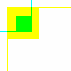
\includegraphics{figures/visual-test-1.png}}
        \end{minipage}
        &
        \begin{minipage}{.3\textwidth}
            \centering
            \frame{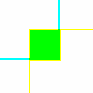
\includegraphics{figures/visual-test-2.png}}
        \end{minipage}
    \end{tabular}
    \caption{Le due immagini di test sovrapposte utilizzando le tre modalit\`a. A sinistra il metodo centrale, nel mezzo il metodo del baricentro, e a destra il metodo inerziale.}
    \label{fig:visual_jaccard_test}
\end{figure}
\chapter{Esperimenti}\label{ch:experiments}

Per confrontare le varie modalit\`a e avere una misura di quali siano le migliori non possiamo basarci solamente su analisi generali, ma dobbiamo fare degli esperimenti.

Per gli esperimenti verranno usate come confronti le lettere in figura \ref{fig:letters}.

\begin{figure}
    \centering
    \begin{tabular}{c|c|c}
        & \emph{d} & \emph{s} \\ \hline
        dritta 
        & 
        \begin{minipage}{.3\textwidth}
            \centering
            
\includegraphics{figures/D_dritta.png}
        \end{minipage}
        & 
        \begin{minipage}{.3\textwidth}
            \centering
            
\includegraphics{figures/S_dritta.png}
        \end{minipage}
        \\ \hline
        tonda 
        & 
        \begin{minipage}{.3\textwidth}
            \centering
            
\includegraphics{figures/D_tonda.png}
        \end{minipage}
        & 
        \begin{minipage}{.3\textwidth}
            \centering
            
\includegraphics{figures/S_tonda.png}
        \end{minipage}
        
    \end{tabular}
    \caption{Le lettere usate come confronto.}
    \label{fig:letters}
\end{figure}

Per valutare le prestazioni di ciascun algoritmo in maniera automatica viene usato un file .json che accompagna la scannerizzazione dell'immagine. In tale file ci sono indicate delle coordinate per ciascuna lettera di interesse. Per avere un unico punto associato a ciascuna lettera, si trova il punto medio fra quelli forniti, in modo da essere sicuri che questo sia in un punto interno alla lettera.

Per trovare le lettere nel testo viene usata una funzione che riceve in ingresso un immagine sezionata secondo le modalit\`a descritte alla sezione \ref{sect:segmentation}, l'immagine della lettera usata come confronto, l'indice di Jaccard da prendere come valore di soglia e un valore per indicare che modalit\`a usare. Questa funzione dovr\`a dunque restituire una lista di rettangoli che sono i rettangoli contenenti le lettere che superano il test e i relativi valori di Jaccard. Ciascun rettangolo sar\`a rappresentato come una coppia di coordinate che si riferiscono a una coppia di vertici opposti.

\section{Grafici precision recall}

Una volta che abbiamo le rappresentazioni di tutti i rettangoli che l'algoritmo ritiene siano la lettera cercata, possiamo usare la lista di coordinate associate alle lettere corrette per quantificare gli errori dell'algoritmo. In particolare dobbiamo contare le volte in cui l'algoritmo ha creduto che una lettera fosse la stessa del riferimento sbagliandosi (falsi positivi) e le volte in cui ha creduto che una lettera non fosse la stessa del riferimento sbagliandosi (falsi negativi).

Idealmente vorremmo che sia i falsi positivi che i falsi negativi fossero 0. Tuttavia ci\`o \`e difficile da ottenere, in quanto alzando il valore di indice di Jaccard di soglia aumentano i falsi negativi, mentre abbassandolo aumentano i falsi positivi.

Nelle figure da \ref{fig:graph_D_dritta} a \ref{fig:graph_S_tonda} si possono visualizzare le affermazioni fatte precedentemente (i grafici relativi alla connettivit\`a a 8 sono stati omessi perch\'e troppo simili ai corrispondenti per la connettivit\`a a 4). Nei grafici sull'asse delle ascisse c'\`e il recall (o sensibilit\`a) e sull'asse delle ordinate la precision (o predittivit\`a). Le definizioni di queste misure sono date in termini dei veri positivi $V_+$, i falsi positivi $F_+$, i veri negativi $V_-$ e i falsi negativi $F_-$.

\begin{equation*}
    \text{recall} = \frac{V_+}{V_+ + F_-}
\end{equation*}

\begin{equation*}
    \text{precision} = \frac{V_+}{V_+ + F_+}
\end{equation*}

Ci\`o che si deduce da queste definizioni \`e che il recall \`e una misura degli errori intesi come falsi negativi, mentre la precision \`e una misura degli errori intesi come falsi positivi. Il caso ideale sarebbe avere precision e recall entrambi pari ad uno. Dai grafici \`e possibile confrontare i vari metodi per cercare di capire quale sia il migliore, ovvero quello che approssima meglio la curva ideale passante da $(1, 1)$.

\begin{figure}
    \centering
    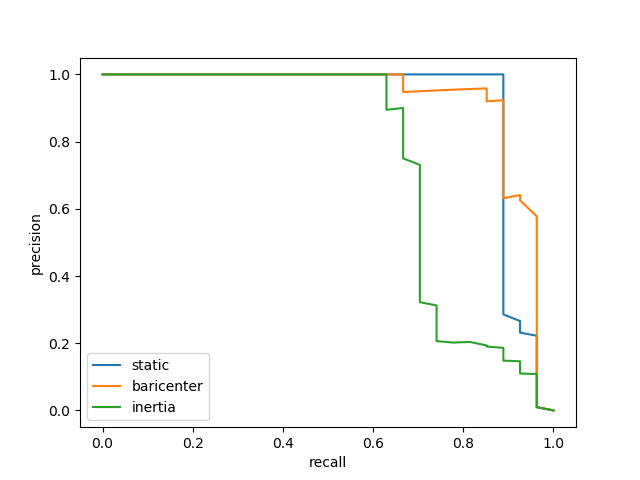
\includegraphics[width=.9\textwidth]{figures/graphs/D_drittaFalse.png}
    \caption{Curve di precision recall per la \emph{d} dritta usando la connettivit\`a a 4.}
    \label{fig:graph_D_dritta}
\end{figure}

\begin{figure}
    \centering
    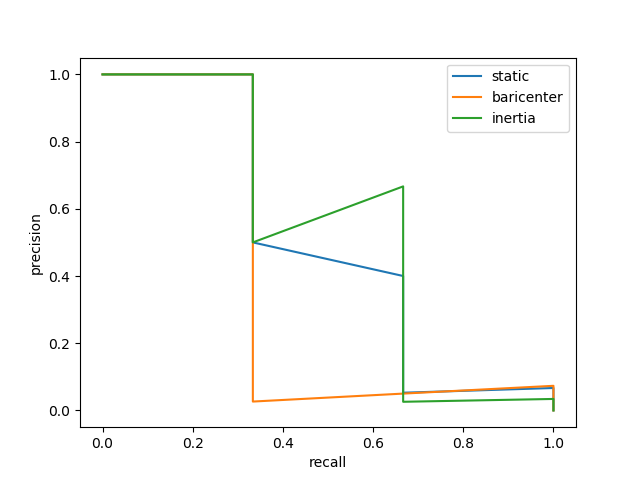
\includegraphics[width=.9\textwidth]{figures/graphs/D_tondaFalse.png}
    \caption{Curve di precision recall per la \emph{d} tonda usando la connettivit\`a a 4.}
    \label{fig:graph_D_tonda}
\end{figure}

\begin{figure}
    \centering
    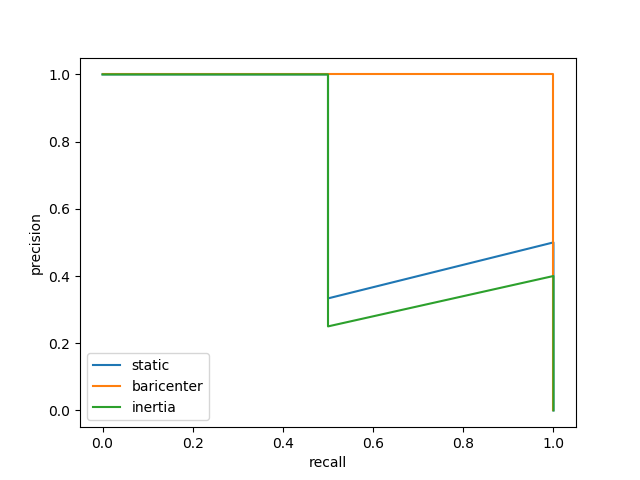
\includegraphics[width=.9\textwidth]{figures/graphs/S_drittaFalse.png}
    \caption{Curve di precision recall per la \emph{s} dritta usando la connettivit\`a a 4.}
    \label{fig:graph_S_dritta}
\end{figure}

\begin{figure}
    \centering
    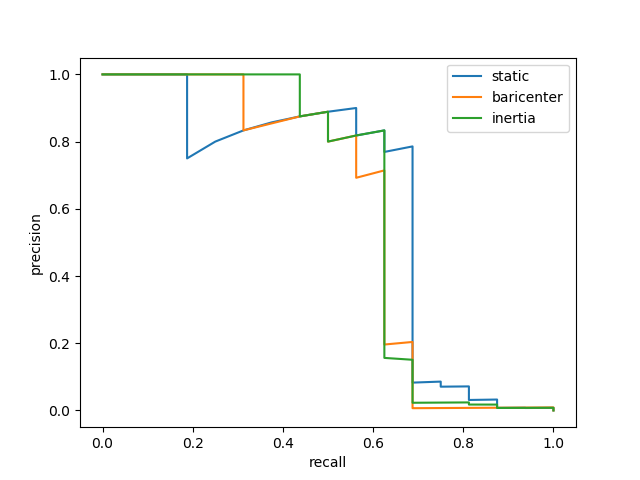
\includegraphics[width=.9\textwidth]{figures/graphs/S_tondaFalse.png}
    \caption{Curve di precision recall per la \emph{s} tonda usando la connettivit\`a a 4.}
    \label{fig:graph_S_tonda}
\end{figure}

\section{Precision interpolata}

I grafici possono essere semplificati facendone quella che viene chiamata interpolazione. In pratica ci si accorge che per alcuni tratti il grafico va ``in salita'', ovvero passa da un punto ad un altro con maggiore recall e precision. Questo significa che il secondo punto \`e migliore al primo secondo ogni misura. Detta in altri termini, usare il valore di soglia per l'indice di Jaccard relativo al secondo punto rispetto a quello del primo punto, comporta l'esclusione di grafemi incorretti, ma non di grafemi corretti e quindi \`e preferibile indiscutibilmente.

Di conseguenza possiamo fare in modo che il primo punto erediti la precision del secondo, in modo da passare dal grafico che indica ``il miglior valore di precision ottenibile per un valore di recall pari a $x$'' a quello che indica ``il miglior valore di precision ottenibile per un valore di recall pari \emph{o maggiore} di $x$''. In questo modo si capisce bene che il grafico interpolato \`e pi\`u interessante.

Formalmente la precision nel grafico interpolato si trova come:
\begin{equation*}
    p_{interp}(r) = \max_{r' \geq r} p(r')
\end{equation*}
Dove $p_{interp}$ \`e la precision interpolata, $p$ la precision, e $r$ un valore di recall.

Nelle figure da \ref{fig:graph_D_dritta_interpolated} a \ref{fig:graph_S_tonda_interpolated} viene raffigurata la versione interpolata dei grafici precision recall.

\begin{figure}
    \centering
    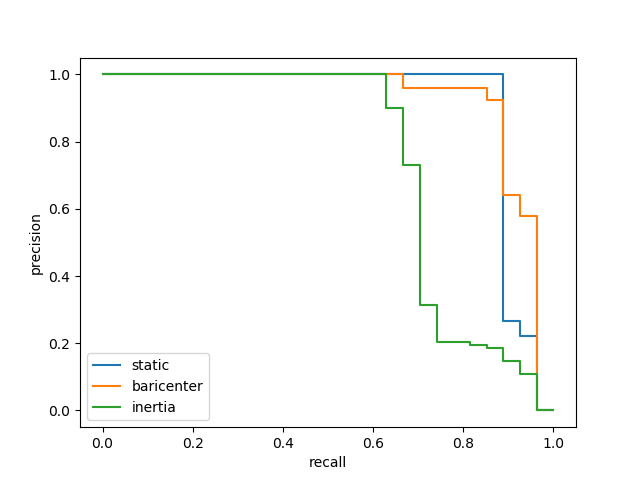
\includegraphics[width=.9\textwidth]{figures/graphs/D_drittaFalseinterpolated.png}
    \caption{Curve di precision recall interpolate per la \emph{d} dritta.}
    \label{fig:graph_D_dritta_interpolated}
\end{figure}

\begin{figure}
    \centering
    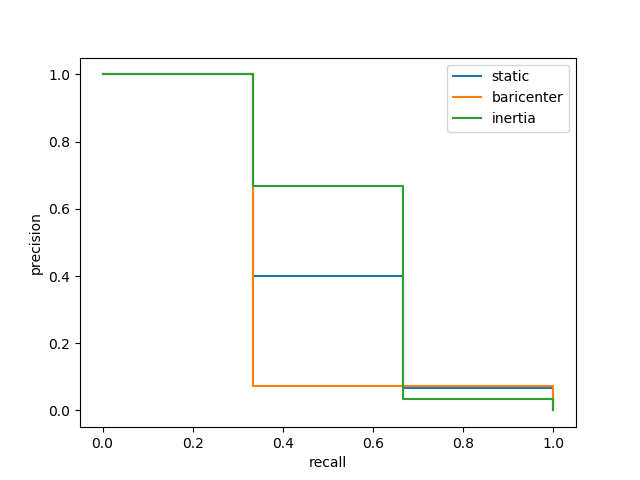
\includegraphics[width=.9\textwidth]{figures/graphs/D_tondaFalseinterpolated.png}
    \caption{Curve di precision recall interpolate per la \emph{d} tonda.}
    \label{fig:graph_D_tonda_interpolated}
\end{figure}

\begin{figure}
    \centering
    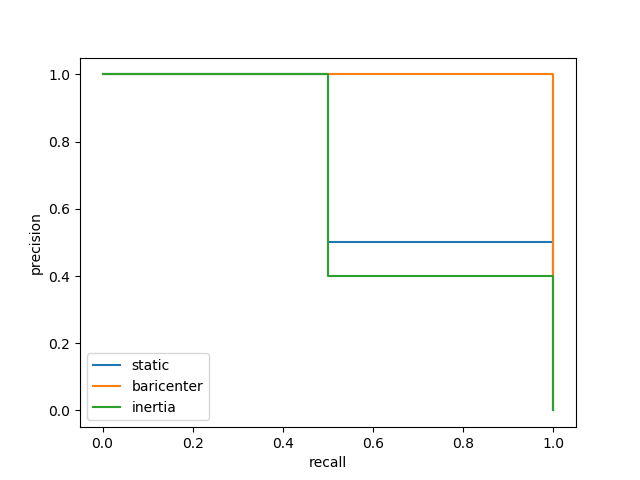
\includegraphics[width=.9\textwidth]{figures/graphs/S_drittaFalseinterpolated.png}
    \caption{Curve di precision recall interpolate per la \emph{s} dritta.}
    \label{fig:graph_S_dritta_interpolated}
\end{figure}

\begin{figure}
    \centering
    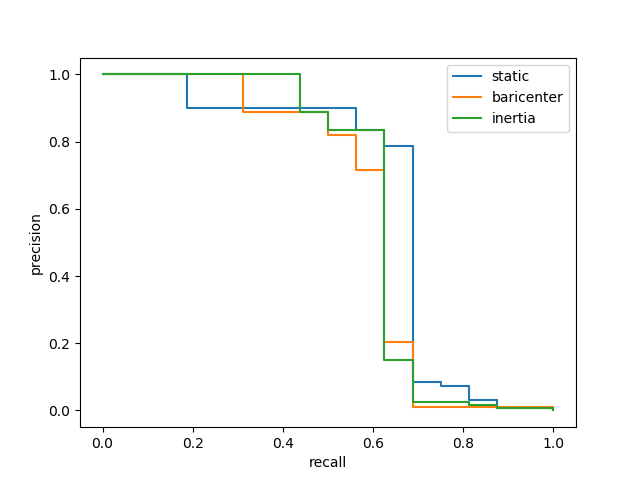
\includegraphics[width=.9\textwidth]{figures/graphs/S_tondaFalseinterpolated.png}
    \caption{Curve di precision recall interpolate per la \emph{s} tonda.}
    \label{fig:graph_S_tonda_interpolated}
\end{figure}

\section{Media fra grafici}

Usare quattro grafici per descrivere un unico metodo \`e eccessivo e dovremmo condensarli in un unico grafico per poter confrontare i metodi pi\`u facilmente. Per fare ci\`o possiamo fare una media fra i grafici delle varie lettere ottenuti con lo stesso metodo per poi confrontare queste medie.

La media non deve essere una media aritmetica standard, poich\'e darebbe eguale peso a tutti i grafemi. Dobbiamo utilizzare una media pesata dove il peso di ciascun grafema \`e dato dalla sua frequenza nel testo. Utilizzando questo approccio, i grafici che otteniamo sono quelli nella figura \ref{fig:graph_all}. Come si evince dalle figure, e come \`e facilmente dimostrabile, la media fra grafici interpolati \`e a sua volta un grafico interpolato e quindi non \`e necessario farne l'interpolazione.

\begin{figure}
    \centering
    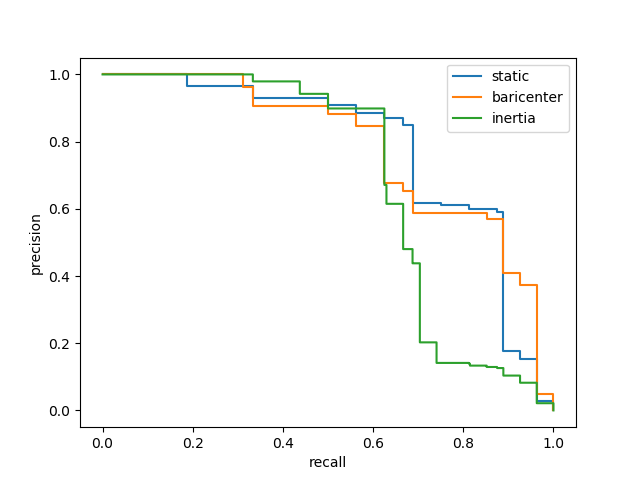
\includegraphics[width=\textwidth]{figures/graphs/False.png}
    \caption{Curve di precision recall medie.}
    \label{fig:graph_all}
\end{figure}

Da questi grafici possiamo notare che il metodo inerziale \`e il migliore per recall bassi, il metodo del baricentro \`e il migliore per recall alti, e il metodo statico \`e il migliore per recall intermedi.

\section{Area}

Dai grafici, anche da quelli complessivi, \`e difficile capire quale metodo sia il migliore in generale. Quello che possiamo fare in questi casi \`e passare da un grafico ad un unico numero. Un modo per fare questo \`e calcolare l'area sottesa dal grafico. Quest'area sar\`a un valore compreso fra 0 e 1 e a metodi migliori corrisponderanno aree maggiori.

Le aree sono facilmente calcolate poich\'e sono semplicemente somme di aree di rettangoli. I loro valori sono riportati in tabella \ref{tab:area}. Come si pu\`o notare i metodi corrispondono a aree simili, tutte vicine a $0.78$, fatta eccezione per il metodo inerziale. Questo \`e probabilmente dovuto al fatto che le lettere sono tutte delle stesse dimensioni, mentre il metodo inerziale \`e efficacie quando le dimensioni sono variabili.

\begin{table}
    \centering
    \begin{tabular}{c|c|c}
        metodo & connettivit\`a 4 & connettivit\`a 8 \\
        \hline
        centrale & \textbf{0.785} & 0.784 \\
        baricentro & 0.782 & 0.781 \\
        inerzia & 0.685 & 0.681 \\
    \end{tabular}
    \caption{Le aree sotto le curve precision recall per tutti i metodi testati. \`E stato evidenziato il valore massimo.}
    \label{tab:area}
\end{table}
\chapter{Interattivit\`a}\label{ch:interactivity}

Un modo semplice per aumentare l'accuratezza del programma \`e renderlo interattivo chiedendo aiuto all'utente per riconoscere le parole. Questo potrebbe sembrare insensato, visto che lo scopo del software \`e riconoscere i grafemi in maniera automatica, tuttavia non \`e cos\`i visto che il programma continuerebbe a fare la maggior parte del lavoro. Infatti, il programma fa tutto il processo descritto nei primi capitoli, fino a individuare le varie lettere e anche scartare quelle che sono molto diverse dal riferimento. L'unica cosa che viene chiesta all'utente \`e individuare i grafemi che corrispondono al riferimento scegliendo fra i pochi che rimangono.

\section{Interfaccia interattiva}

Per quanto riguarda l'interfacciamento con l'utente, questo avviene in modo molto semplice: si apre una finestra che chiede all'utente se la lettera mostrata \`e corretta che, quando l'utente ha risposto, si richiude per mostrarne un'altra. In questo modo l'utente deve fare una sola azione (premere un tasto) per ogni grafema mostrato, quindi viene ridotta al minimo la parte di lavoro non automatizzata.

L'interfaccia che vede l'utente \`e quella di figura \ref{fig:gui}. Nella prima riga c'\`e il comando in cui si dice di premere il tasto \emph{y} (``yes'') se la lettera \`e quella che si sta cercando o il tasto \emph{n} (``no'') in caso contrario. Viene anche mostrato l'indice di Jaccard relativo alla lettera per avere un'informazione aggiuntiva.

\begin{figure}
    \centering
    \frame{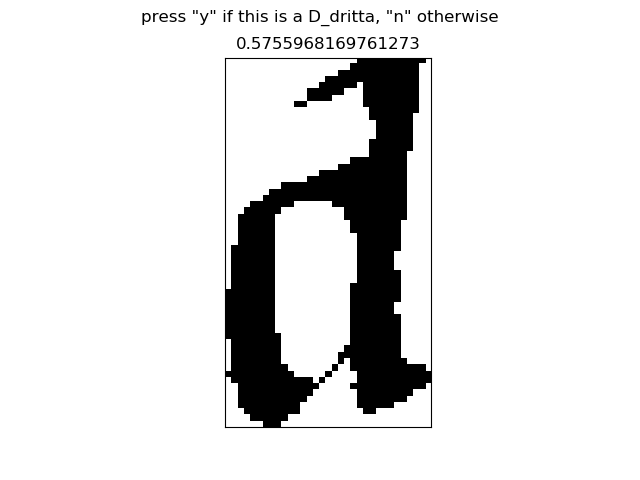
\includegraphics[width=.8\textwidth]{figures/gui.png}}
    \caption{L'interfaccia grafica sviluppata. In alto le indicazioni e l'indice di Jaccard nella seconda riga.}
    \label{fig:gui}
\end{figure}

\section{Interattivit\`a limitata}

Nel caso di documenti molto lunghi, comprendenti dunque molte pagine, chiedere conferma all'utente per ogni lettera, significherebbe chiedergli troppo lavoro. Tuttavia ci\`o non significa che l'interattivit\`a non sia una buona idea.

La soluzione consiste nell'integrare una parte interattiva con una parte completamente automatica. In pratica, durante la parte interattiva si raccolgono nuovi riferimenti che verranno poi utilizzati nella parte completamente automatica. Questo significa che nel primo round verranno selezionate soltanto alcune lettere. Per scegliere le lettere da usare nel primo round \`e necessario usare un generatore di numeri casuali, altrimenti si possono avere effetti indesiderati (se, ad esempio, analizziamo solamente una pagina potrebbe succedere che la grafia di pagine successive sia diversa da quella della pagina selezionata).

\subsection{Tipi di media}

Una volta che abbiamo l'insieme di riferimenti trovati in maniera casuale e interattiva, possiamo calcolare, per ogni nuova lettera, gli indici di Jaccard relativi a ciascun riferimento. Adesso per\`o dobbiamo trovare un modo per passare da tanti valori ad uno solo indicativo di tutti.

Ci\`o che stiamo cercando \`e una funzione che faccia da media. Potremmo pensare di usare la media aritmetica, ma questa non ha certe propriet\`a che stiamo cercando. Infatti vogliamo che la funzione restituisca 1 quando almeno uno degli elementi \`e 1. Questo perch\'e il fatto che uno dei valori sia 1 equivale a dire che la lettera che stiamo testando \`e identica ad un riferimento e perci\`o \`e corretta sicuramente.

A questo punto potremmo pensare di usare come media la funzione \emph{max}, che restituisce il massimo dei valori in ingresso. Questa funzione ha infatti la propriet\`a di cui abbiamo parlato prima: se 1 \`e fra i valori in ingresso, allora \emph{max} restituir\`a sicuramente 1 (ricordiamo che i valori di ingresso sono indici di Jaccard e perc\`o sono sempre compresi fra 0 e 1 inclusi). Tuttavia, neanche questa funzione \`e adatta, poich\'e non tiene conto dei valori pi\`u bassi. Questo \`e un problema perch\'e passare da una lista di valori $(\frac{1}{2})$ a $(\frac{1}{2}, \frac{1}{4})$ deve far diminuire l'indice risultante.

Dopo queste considerazioni arriviamo alla seguente formula.
\begin{equation*}
    1 - \prod_{0\leq i < n} (1-x_i)
\end{equation*}
In cui $n$ \`e il numero di valori in ingresso. Con questa funzione tutti i valori contribuiscono al risultato finale a meno che uno dei valori sia 1, in qual caso il risultato \`e 1. Ancora per\`o non \`e perfetta come funzione, infatti se prendo $A = ( \frac{1}{2}, \frac{1}{2} )$, il risultato non \`e $\frac{1}{2}$ come sarebbe ovvio aspettarsi, ma $\frac{3}{4}$.

Dopo un ultimo ritocco alla formula, si arriva alla forma seguente.
\begin{equation*}
    1 - \sqrt[n]{\prod_{0\leq i < n} (1-x_i)}
\end{equation*}
Questa ha tutte le propriet\`a della funzione precedente e in pi\`u, se tutti i valori sono uguali, restituisce il valore in ingresso.

\section{Confronto con modalit\`a non interattiva}

Per verificare se l'introduzione di interattivit\`a ha aiutato il programma dobbiamo confrontarne i risultati con quelli che ottenevamo senza interattivit\`a. Nelle figure \ref{fig:graph_total_static}, \ref{fig:graph_total_baricenter} e \ref{fig:graph_total_inertia} sono mostrati i grafici precision recall per le varie modalit\`a.

\begin{figure}
    \centering
    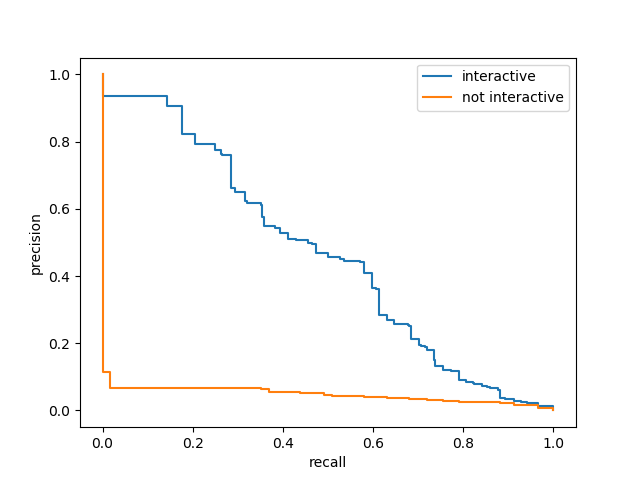
\includegraphics[width=.9\textwidth]{figures/graphs/totalstaticFalse.png}
    \caption{Curve precision recall con e senza interattivit\`a, metodo centrale.}
    \label{fig:graph_total_static}
\end{figure}

\begin{figure}
    \centering
    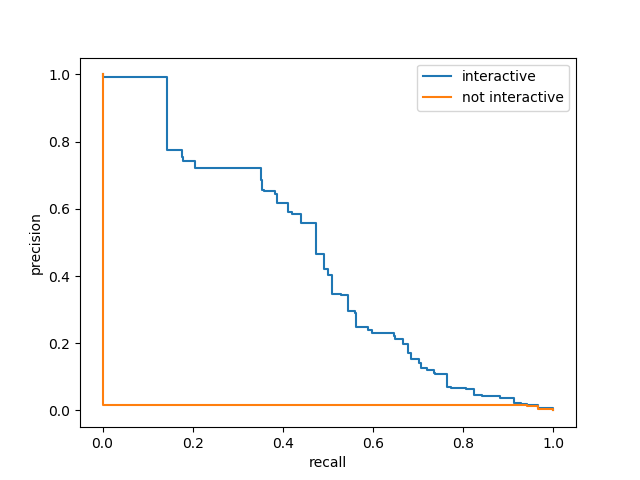
\includegraphics[width=.9\textwidth]{figures/graphs/totalbaricenterFalse.png}
    \caption{Curve precision recall con e senza interattivit\`a, metodo del baricentro.}
    \label{fig:graph_total_baricenter}
\end{figure}

\begin{figure}
    \centering
    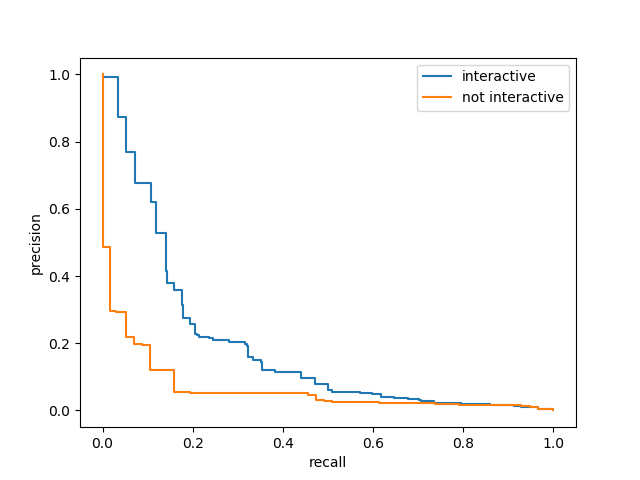
\includegraphics[width=.9\textwidth]{figures/graphs/totalinertiaFalse.png}
    \caption{Curve precision recall con e senza interattivit\`a, metodo inerziale.}
    \label{fig:graph_total_inertia}
\end{figure}

Come si nota nelle figure, le curve relative alla non interattivit\`a sono diverse rispetto a quelle del capitolo precedente. Questo perch\'e sono state utilizzate pagine diverse per enfatizzare il punto forte dell'interattivit\`a: \`e efficace con pagine scritte con calligrafie diverse.

\`E evidente come il metodo inerziale sia il peggiore dei tre in questa modalit\`a. Infatti anche in questo caso le lettere sono tutte della stessa grandezza pi\`u o meno. Si faccia caso, per\`o, al fatto che il metodo inerziale \`e il migliore nella modalit\`a non interattiva. Questo \`e dovuto al fatto che, come avevamo predetto nella sezione \ref{ssect:jaccard}, questo metodo \`e adatto ai casi in cui le pagine hanno stili differenti e in particolare hanno lettere di dimensione variabile.

Come prima, mostriamo anche le misure delle aree sotto le curve di precision recall nella tabella \ref{tab:area_interactive}. Va ricordato che questi valori non sono deterministici come quelli del capitolo \ref{ch:experiments}, ma dipendono dalla scelta casuale delle lettere estratte e usate per l'interattivit\`a.

\begin{table}
    \centering
    \begin{tabular}{c|c|c|c}
        connettivit\`a & modalit\`a & interattivo & non interattivo  \\
        \hline
        \multirow{3}{1em}{4} & centro & 0.463 & 0.047 \\
        & baricentro & 0.448 & 0.017 \\
        & inerzia & 0.188 & 0.063 \\
        \hline
        \multirow{3}{1em}{8} & centro & 0.449 & 0.046 \\
        & baricentro & 0.391 & 0.017 \\
        & inerzia & 0.193 & 0.063 \\
    \end{tabular}
    \caption{Le aree sotto le curve precision recall per tutti i metodi interattivi testati e il confronto rispetto agli stessi metodi senza interattivit\`a.}
    \label{tab:area_interactive}
\end{table}
\chapter{Conclusioni}\label{ch:conclusioni}

Quello che abbiamo fatto \`e stato, a partire da digitalizzazioni di documenti manoscritti medievali, trovare un metodo per l'estrazione di alcuni grafemi che ci interessavano.

Prima di tutto abbiamo binarizzato le immagini per rendere pi\`u semplici le operazioni successive. Dopodich\'e abbiamo utilizzato metodi basati su proiezioni orizzontali e verticali per suddividere il documento nelle righe e nei caratteri che lo compongono.

Una volta isolate le varie immagini dei caratteri e estratti da essi i grafemi mediante lo studio delle componenti connesse, siamo passati a confrontarle con dei modelli estratti manualmente in precedenza per trovare quelle che rappresentano ciascuno dei grafemi che ci interessano.

Il confronto avviene mediante vari passaggi successivi. Inizialmente si trasformano le immagini per renderle tutte delle stesse dimensioni. Questo avviene secondo varie modalit\`a che verranno confrontate fra di loro. Infine si confrontano le immagini tramite l'indice di Jaccard.

Per confrontare la bont\`a delle varie modalit\`a si usano degli scan gi\`a analizzati manualmente. I risultati degli esperimenti sono riportati nel capitolo \ref{ch:experiments}, da cui si vede che tutte le modalit\`a si comportano in maniera molto simile, con piccole differenze.

Come ultima cosa si \`e usata un'interfaccia interattiva per rendere il programma migliore in situazioni in cui non basta un unico modello per analizzare tutto il documento. Questo \`e stato descritto nel capitolo \ref{ch:interactivity}, in cui si pu\`o vedere il miglioramento considerevole rispetto alla modalit\`a non interattiva.

In conclusione, il programma risulta utile per la ricerca dei grafemi che ci interessavano e si rivela anche versatile tramite l'uso della modalit\`a interattiva, nonostante l'apparente semplicit\`a delle tecniche utilizzate.

\addcontentsline{toc}{chapter}{Bibliografia}
%\bibliographystyle{plain}
\bibliography{files/biblio}
\bibliographystyle{unsrt}
%\bibliography{sp,xml}

\end{document} 